\documentclass[conference]{IEEEtran}

\usepackage{amsmath}
\usepackage{booktabs}
\usepackage{graphicx}
\usepackage{microtype}
\usepackage{siunitx}
\usepackage{url}

\graphicspath{{../reports/figures/}}
\sisetup{detect-weight=true,detect-family=true}

\title{S8-CFD: A Lightweight From-Scratch Context-Fused Detector for Small Drone Detection}

\author{\IEEEauthorblockN{Hardefa Rogonondo}}

\begin{document}
\maketitle

\begin{abstract}
This report presents S8-CFD, a lightweight single-class drone detector designed
and implemented from scratch in PyTorch. The dataset and problem setting
emphasize small-object localization: all source images are 2560$\times$1440,
contain annotated drones, and are grouped to reduce leakage from related
sequential and raw/augmented samples. S8-CFD uses a stride-8 anchor-free prediction grid with S8/S16/S32
context fusion, GroupNorm, custom decoding, and custom non-maximum suppression.
The final baseline obtains validation AP50/AP75/mAP50-95 of
0.9376/0.4038/0.4792 and sealed-test AP50/AP75/mAP50-95 of
0.8811/0.3026/0.4115. At the validation-selected threshold of 0.999, sealed-test
precision, recall, and F1 are 0.9437, 0.8584, and 0.8990. A standard IoU-loss
ablation improves validation AP50 and operating F1 slightly, but does not
improve AP75 or the predetermined validation mAP50-95 selection metric.
\end{abstract}

\section{Introduction}
Small drones are visually compact and often appear against sky, buildings, or
natural scenery. This makes coarse detection easier than precise localization:
the frozen baseline has high AP50 but much lower AP75, motivating a careful
localization-focused analysis. The implementation is intentionally developed
from scratch without pretrained detector weights, YOLO/Ultralytics, torchvision
detector models, timm backbones, or imported detection architectures.

The resulting model, S8-CFD, is a 3,242,589-parameter anchor-free detector. It
uses stride-8 small-object prediction and fuses S8, S16, and S32 feature context
in a custom head. The implementation includes from-scratch target encoding,
decoding, IoU computation, and NMS. PyTorch is used as the tensor and training
framework \cite{paszke2019pytorch}; GroupNorm follows the normalization choice
of Wu and He \cite{wu2018group}. Multi-scale context fusion is related in spirit
to feature pyramid reasoning \cite{lin2017feature}, but the architecture here is
not an imported FPN detector.

\section{Dataset and Evaluation Protocol}
The dataset contains 2400 source images and 4800 annotated objects. Each image is
2560$\times$1440 and the annotation set has one semantic class: drone. Although
the dataset contains two annotated drones per image, the detector and inference
code do not hard-code two detections; inference emits a variable number of
post-NMS predictions.

The split is grouped to reduce leakage from related samples. A
filename-derived \texttt{capture\_pair} field is used as an inferred proxy for
source identity or sequential relation, not as ground-truth identity. Train,
validation, and test groups are separated to reduce overlap from sequentially
related samples and raw/augmented variants. Table~\ref{tab:data} summarizes the
frozen split.

\begin{table}[t]
\centering
\caption{Frozen dataset split.}
\label{tab:data}
\begin{tabular}{lrr}
\toprule
Split & Images & Objects \\
\midrule
Train & 1696 & 3392 \\
Validation & 245 & 490 \\
Test & 459 & 918 \\
\midrule
Total & 2400 & 4800 \\
\bottomrule
\end{tabular}
\end{table}

The test set remained sealed until the final model, checkpoint, and operating
threshold were frozen. The final model is the validation-best S8-CFD baseline at
epoch 19, selected by validation mAP50-95. AP is computed from ranked candidates
retained at \texttt{EVAL\_CONFIDENCE\_FLOOR}=0.001, following the standard
ranked detection-evaluation convention used in COCO-style AP analysis
\cite{lin2014microsoft}. Precision, recall, and F1 are computed at an operating
confidence threshold. The final threshold 0.999 was selected on validation only.
NMS IoU is 0.50, \texttt{EVAL\_TOP\_K}=500, and
\texttt{MAX\_DETECTIONS}=100. The sealed test was evaluated once after freezing
the model and threshold.

\section{S8-CFD Detector}
Input images are resized to 960$\times$540 and vertically padded to a
960$\times$544 canvas. S8-CFD predicts on a stride-8 68$\times$120 grid. Each
cell outputs five values: an objectness logit, $x/y$ cell offsets, and log
width/height. Positive cells are assigned by object centers.

The model uses custom convolutional blocks with GroupNorm and context fusion
from S8, S16, and S32 feature levels. The detection head is anchor-free: decoded
centers use sigmoid-normalized cell offsets, sizes use exponentiated log
width/height, and boxes are converted to normalized \texttt{xyxy} coordinates.
NMS is implemented in PyTorch tensor operations rather than through an external
library. Figure~\ref{fig:architecture} summarizes the implemented architecture.

The baseline objective is
\begin{equation}
L_{\mathrm{base}} = L_{\mathrm{obj}} + 5L_{\mathrm{center}} + 2L_{\mathrm{size}},
\end{equation}
where objectness is balanced binary cross entropy over positive and negative
cells, and center and size terms use Smooth L1. Training uses AdamW
\cite{loshchilov2019decoupled}.

The localization ablation adds a standard IoU term for positive assigned cells:
\begin{equation}
L_{\mathrm{exp}} = L_{\mathrm{base}} + \lambda_{\mathrm{iou}}L_{\mathrm{iou}},
\quad \lambda_{\mathrm{iou}}=1,
\end{equation}
\begin{equation}
L_{\mathrm{iou}} = 1-\mathrm{IoU}.
\end{equation}
No GIoU, DIoU, or CIoU variant is used in this ablation.

\begin{figure}[t]
\centering
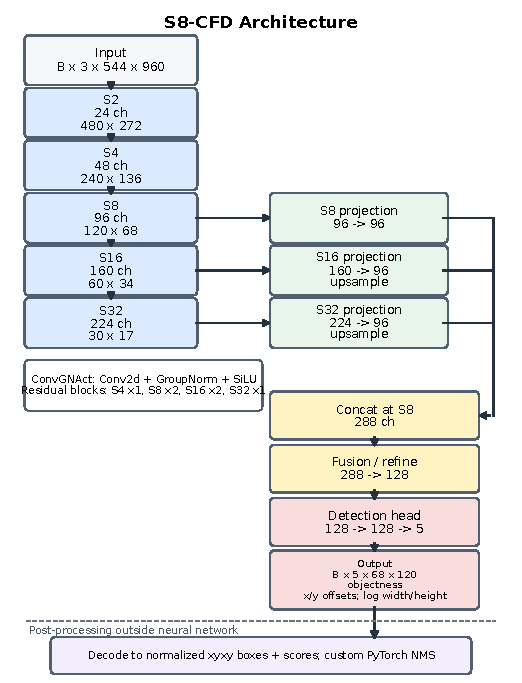
\includegraphics[width=\columnwidth]{s8_cfd_architecture.pdf}
\caption{S8-CFD architecture. Features from strides 8, 16, and 32 are projected
and fused at stride 8 before the anchor-free detection head.}
\label{fig:architecture}
\end{figure}

\section{Experiments and Results}
The reference baseline configuration is fixed for 20 epochs, batch size 2,
learning rate 0.001, weight decay 0.0001, no learning-rate scheduler, and seed
42. Training used Windows CUDA on an NVIDIA GTX 1660 SUPER with
\texttt{NUM\_WORKERS}=4. W\&B tracking was used for experiment logging, while
the repository also supports CPU Docker smoke runs and platform-aware
CUDA/MPS/CPU local execution.

Table~\ref{tab:results} gives the compact validation and final sealed-test
summary. For the IoU ablation, AP metrics come from the validation-best
checkpoint, while precision, recall, and F1 use the validation-selected
threshold from the threshold-sweep artifact.

\begin{table*}[t]
\centering
\caption{Main validation and sealed-test results. AP uses ranked candidates;
P/R/F1 use each listed operating threshold.}
\label{tab:results}
\begin{tabular}{lrrrrrrrr}
\toprule
Run & Epoch & Threshold & AP50 & AP75 & mAP & Prec. & Rec. & F1 \\
\midrule
Baseline validation & 19 & 0.999 & 0.9376 & 0.4038 & 0.4792 & 0.9611 & 0.9082 & 0.9339 \\
IoU $\lambda=1$ validation & 17 & 0.998 & 0.9507 & 0.4023 & 0.4784 & 0.9261 & 0.9469 & 0.9364 \\
Final sealed test & 19 & 0.999 & 0.8811 & 0.3026 & 0.4115 & 0.9437 & 0.8584 & 0.8990 \\
\bottomrule
\end{tabular}
\end{table*}

\begin{figure}[t]
\centering
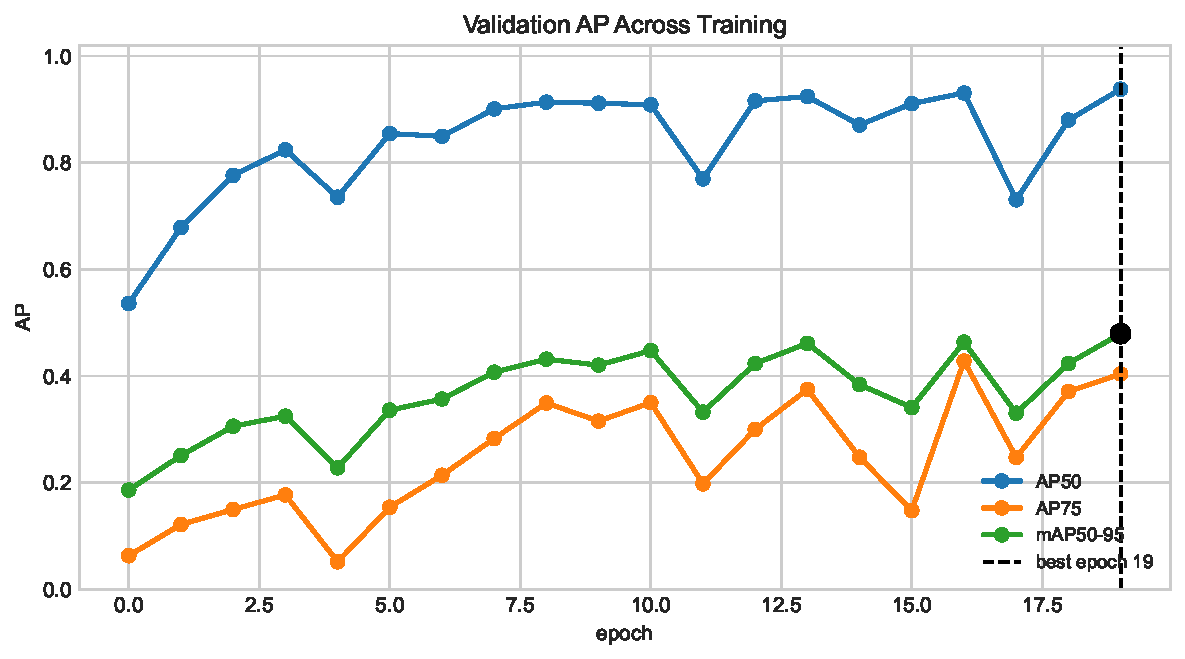
\includegraphics[width=\columnwidth]{baseline_s8_cfd_validation_ap.pdf}
\caption{Baseline validation AP curves. The validation-best checkpoint is
selected by mAP50-95, not by operating F1.}
\label{fig:apcurve}
\end{figure}

The IoU ablation is neutral to negative with respect to the predetermined
selection metric. It improves validation AP50 from 0.9375629425 to
0.9507038593 and slightly improves operating F1 from 0.9338929696 to
0.9364278507. However, AP75 decreases from 0.4037680626 to 0.4022931159, and
mAP50-95 decreases from 0.4791892208 to 0.4783972635. The mAP difference is only
about 0.0008, so it should not be overstated; nevertheless, the ablation does
not improve the predetermined validation criterion. The baseline therefore
remains the final selected model.

The sealed-test evaluation of the frozen baseline contains 459 images and 918
objects. At threshold 0.999 it produces 788 true positives, 47 false positives,
and 130 false negatives, with 835 displayed predictions or 1.819 predictions per
image. Relative to validation, sealed-test AP50 changes by -0.05645, AP75 by
-0.10117, mAP50-95 by -0.06766, and F1 by -0.03486.

\section{Discussion and Limitations}
The final detector achieves AP50 of 0.8811 and operating precision of 0.9437 on
the sealed test split.
Performance decreases relative to validation, especially at AP75. This supports
the interpretation that stricter localization generalizes less strongly than
AP50-level detection. Held-out capture-pair conditions may contribute to the
gap, but the evidence does not establish causality and should not be labeled
definite overfitting.

\begin{figure*}[!t]
\centering
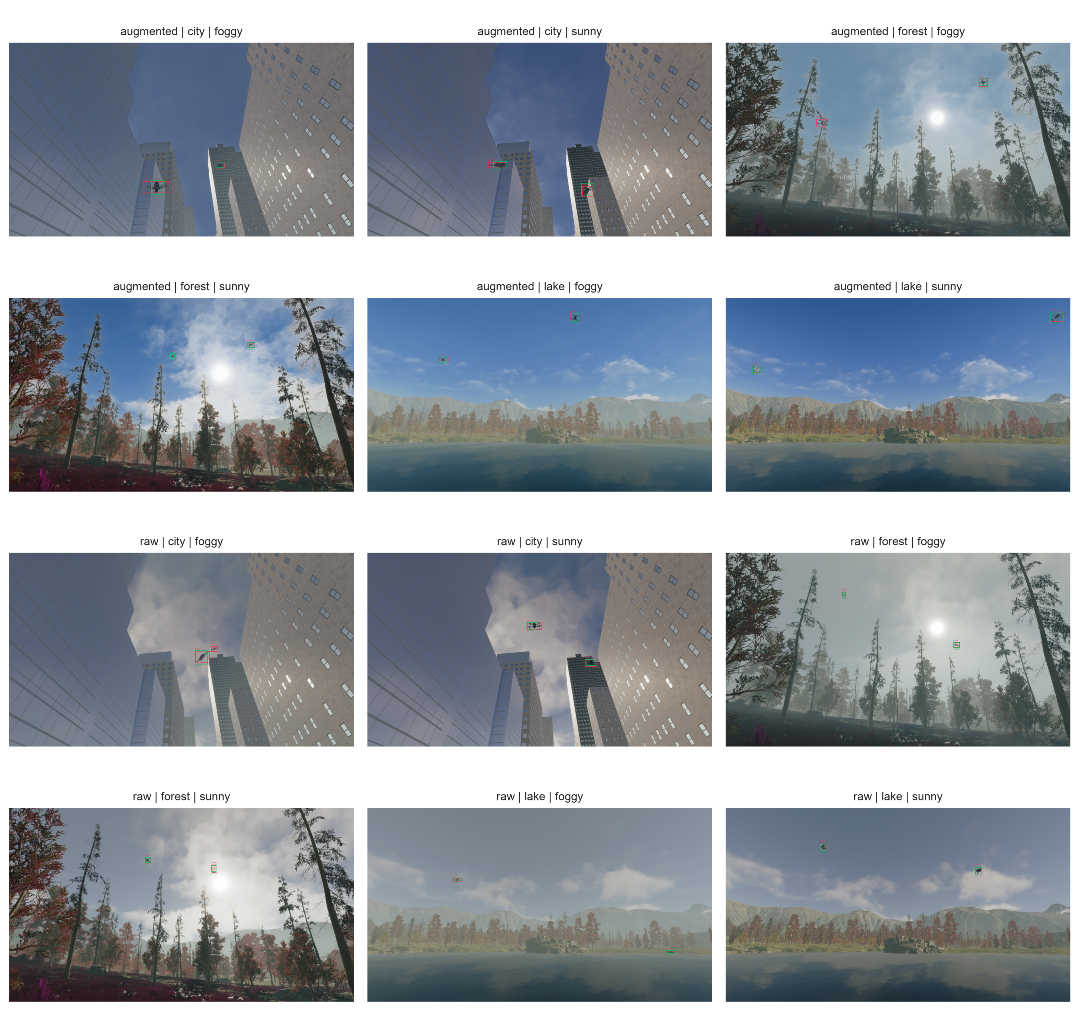
\includegraphics[width=0.66\textwidth]{final_evaluation_qualitative_examples_paper.pdf}
\caption{Representative sealed-test predictions. The 12-image subset
was curated for coverage across raw/augmented, city/forest/lake, and
sunny/foggy conditions, not for correctness or confidence.}
\label{fig:qual}
\end{figure*}

Several limitations remain. The dataset is relatively small, single-class, and
structured around inferred filename metadata. The split grouping is a practical
leakage-reduction proxy rather than verified scene identity. The main training
results use one primary seed. The IoU experiment tests only standard IoU with
$\lambda_{\mathrm{iou}}=1$; it does not exhaust localization-loss choices. The
results do not imply broad real-world deployment readiness.

\section{Conclusion}
S8-CFD demonstrates that a compact, from-scratch, context-fused anchor-free
detector can provide useful drone detection under a leakage-aware validation and
sealed-test protocol. The final selected baseline achieves sealed-test
AP50/AP75/mAP50-95 of 0.8811/0.3026/0.4115 and precision/recall/F1 of
0.9437/0.8584/0.8990 at the frozen validation-selected threshold. A standard
IoU-loss ablation did not improve the predetermined validation mAP50-95
criterion, so it serves as useful neutral/negative evidence rather than a new
selected model. Implementation, final weights, frozen experiment artifacts,
Docker CPU smoke support, and executed notebooks are included in the repository.

\bibliographystyle{IEEEtran}
\bibliography{references}

\end{document}
